\documentclass{beamer}
\usepackage[utf8]{inputenc}
\usepackage{clrscode}
\usepackage{multicol}
\setbeamertemplate{navigation symbols}{}
\usetheme{Boadilla}
\title{Algorithms for Longest Common Extensions}
\author{Jesper Kristensen}
\institute[DTU Informatics]{DTU Informatics\\Technical University of Denmark}
\date{August 31, 2011}
\begin{document}

\newcommand{\sortt}{\textit{sort}(n,\sigma)}
\newcommand{\LCE}{\textit{LCE}}
\newcommand{\NCA}{\textit{NCA}}
\newcommand{\RMQ}{\textit{RMQ}}
\newcommand{\SA}{\textit{SA}}
\newcommand{\SAinv}{\textit{SA}^{-1}} % math
\newcommand{\SAi}{SA$^{-1}$} % no math
\newcommand{\LCP}{\textit{LCP}}
\newcommand{\LA}{\textit{LA}}
\newcommand{\suff}{\textit{suff}}
\newcommand{\logceil}{\lceil\log n\rceil}
\newcommand{\fprint}[1][k]{\ensuremath{\proc{Fingerprint}_{#1}}}
\newcommand{\fprintk}{\fprint[k]}
\newcommand{\RMQpq}[2]{RMQ\textless$#1$, $#2$\textgreater}
\newcommand{\RMQn}{\RMQpq{1}{n}}
\newcommand{\RMQq}{\RMQpq{n}{1}}
\newcommand{\RMQlog}{\RMQpq{n}{\log n}}

\begin{frame}
\titlepage
\end{frame}

\begin{frame}{Contents}
\tableofcontents
\end{frame}

\section{Introduction}
\subsection{The LCE Problem}
\begin{frame}{The LCE Problem and the \proc{DirectComp} algorithm}
    \begin{block}{Input}
        \begin{itemize}
            \item $s=abbababba$
            \item $(i,j)=(4,6)$
        \end{itemize}
    \end{block}
    \begin{block}{The \proc{DirectComp} algorithm}
        %\setlength{\unitlength}{1cm}
        \definecolor{matchcolor}{rgb}{.6,1,.6}
        \definecolor{mismatchcolor}{rgb}{1,.6,.6}
        \begin{picture}(300,50)
            \put(0, 30){\makebox(20, 20){$s=$}}
            \put(20, 30){\framebox(20, 20){a}}
            \put(40, 30){\framebox(20, 20){b}}
            \put(60, 30){\framebox(20, 20){b}}
            \put(80, 30){\framebox(20, 20){a}}
            \put(100, 30){\framebox(20, 20){b}}
            \put(120, 30){\framebox(20, 20){a}}
            \put(140, 30){\framebox(20, 20){b}}
            \put(160, 30){\framebox(20, 20){b}}
            \put(180, 30){\framebox(20, 20){a}}
            \uncover<2-2>{
                \put(200, 30){\makebox(100, 20){1 match}}
                \put(80,30){\framebox(20, 20){\colorbox{matchcolor}{\makebox(13,14){a}}}}
                \put(90, 15){\vector(0,1){13}}
                \put(80, 0){\makebox(20, 15){4}}
                \put(120,30){\framebox(20, 20){\colorbox{matchcolor}{\makebox(13,14){a}}}}
                \put(130, 15){\vector(0,1){13}}
                \put(120, 0){\makebox(20, 15){6}}
            }
            \uncover<3->{
                \put(200, 30){\makebox(100, 20){2 matches}}
            }
            \uncover<3-3>{
                \put(100,30){\framebox(20, 20){\colorbox{matchcolor}{\makebox(13,14){b}}}}
                \put(110, 15){\vector(0,1){13}}
                \put(100, 0){\makebox(20, 15){5}}
                \put(140,30){\framebox(20, 20){\colorbox{matchcolor}{\makebox(13,14){b}}}}
                \put(150, 15){\vector(0,1){13}}
                \put(140, 0){\makebox(20, 15){7}}
            }
            \uncover<4-4>{
                \put(120,30){\framebox(20, 20){\colorbox{mismatchcolor}{\makebox(13,14){a}}}}
                \put(130, 15){\vector(0,1){13}}
                \put(120, 0){\makebox(20, 15){6}}
                \put(160,30){\framebox(20, 20){\colorbox{mismatchcolor}{\makebox(13,14){b}}}}
                \put(170, 15){\vector(0,1){13}}
                \put(160, 0){\makebox(20, 15){8}}
            }
        \end{picture}
    \end{block}
    \uncover<5->{
        \begin{block}{Result}
            $LCE_s(4,6)=2$
        \end{block}
    }
\end{frame}

\subsection{The \proc{DirectComp} algorithm}
\begin{frame}{Existing Algorithm: \proc{DirectComp}}
    \begin{tabular}{r l}
        Preprocessing & $O(1)$ \\
        Space & $O(1)$ \\
        Query & $O(|\LCE(i,j)|)=O(n)$ \\
        Average query & $O(1)$ \\
    \end{tabular}

    \vspace{1cm}
    For a string length $n$ and alphabet size $\sigma$, the average LCE value over all $n^\sigma$ strings and $n^2$ query pairs is $O(1)$.
\end{frame}

\section{Existing Results}
\subsection{The \proc{SuffixNca} Algorithm}
\begin{frame}{Existing Algorithm: \proc{SuffixNca}}
    $\LCE_s(i,j) = D[\NCA_\mathcal{T}(L_i,L_j)]$
\end{frame}

\subsection{The \proc{LcpRmq} Algorithm}
\begin{frame}{Existing Algorithm: \proc{LcpRmq}}
    \begin{multicols}{2}{
        \begin{align*}
            s&=abbababba\\
            s[2\twodots n]&=bbababba\\
            s[3\twodots n]&=bababba\\
            \LCE_s(2,3)&=1
        \end{align*}
        \newpage
        \begin{center}
            \uncover<2->{
                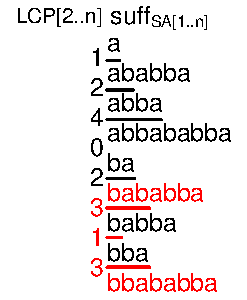
\includegraphics[width=0.26\textwidth,page=1]{../doc/sa+lcp+min.pdf}
            }
        \end{center}
    }
    \end{multicols}
    \uncover<3->{
        \begin{center}
            $\LCE(i,j)=\LCP[\RMQ_{\LCP}(\SAinv[i] + 1, \SAinv[j])]$\\
            where $\SAinv[i] < \SAinv[j]$\\
            \vspace{1em}
            \begin{tabular}{r l}
                Preprocessing & $O(\sortt)$ \\
                Space & $O(n)$ \\
                Query & $O(1)$ \\
                Average query & $O(1)$ \\
            \end{tabular}
        \end{center}
    }
\end{frame}

\section{The \fprintk\ Algorithm}
\subsection{Data Structure}
\begin{frame}{The \fprintk\ Algorithm: Data Structure}
    \begin{itemize}
        \item For a string $s[1\twodots n]$, the $t$-length fingerprints $F_t[1\twodots n]$ are natural numbers, such that $F_t[i] = F_t[j]$ if and only if $s[i\twodots i+t+1] = s[j\twodots j+t+1]$.
        \item For each of $k$ levels, $\ell = 0\twodots k-1$:
        \begin{itemize}
            \item $t_\ell = \Theta(n^{\ell/k}), t_0=1$
            \item $H_\ell = F_{t_\ell}$
        \end{itemize}
    \end{itemize}
    \begin{center}
        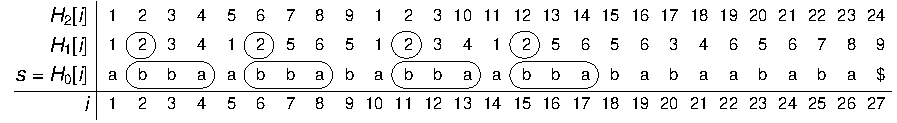
\includegraphics[width=0.98\textwidth,page=1]{../doc/fingerprint.pdf}
    \end{center}
    \begin{tabular}{r l}
        Space & $O(k\cdot n)$\\
    \end{tabular}
\end{frame}

\subsection{Query}
\begin{frame}{The \fprintk Algorithm: Query}
    \begin{enumerate}
        \item As long as $H_\ell[i+v] = H_\ell[j+v]$, increment $v$ by $t_\ell$, increment $\ell$ by one, and repeat this step unless and $\ell = k-1$.
        \item As long as $H_\ell[i+v] = H_\ell[j+v]$, increment $v$ by $t_\ell$ and repeat this step.
        \item Stop and return $v$ when $\ell = 0$, otherwise decrement $\ell$ by one and go to step two.
    \end{enumerate}
    \begin{center}
        \includegraphics[width=0.8\textwidth,page=2]{../doc/fingerprint.pdf}\\
         $\LCE(3,12)$
    \end{center}
    \begin{tabular}{r l}
        Query & $O(k\cdot n^{1/k})$ \\
        Average query & $O(1)$ \\
    \end{tabular}
\end{frame}

\end{document}

